\subsection{Low BDT Score Sidebands}
\label{sec:LowBDTScoreSidebands}

The second set of sub-sidebands to inspect is obtained by selecting the low BDT scoring regions of the far sidebands. In the case of the 1eNp selection, this corresponds to the region with $\pi^0$ scores and non-$\pi^0$ scores both less than 0.1, while for the 1e0p selection, we require a background score less than 0.4. These sidebands are illustrated in Figure~\ref{fig:LowBDTSideband}.

\begin{figure}[H]
    \centering
    \begin{subfigure}{0.5\linewidth}
        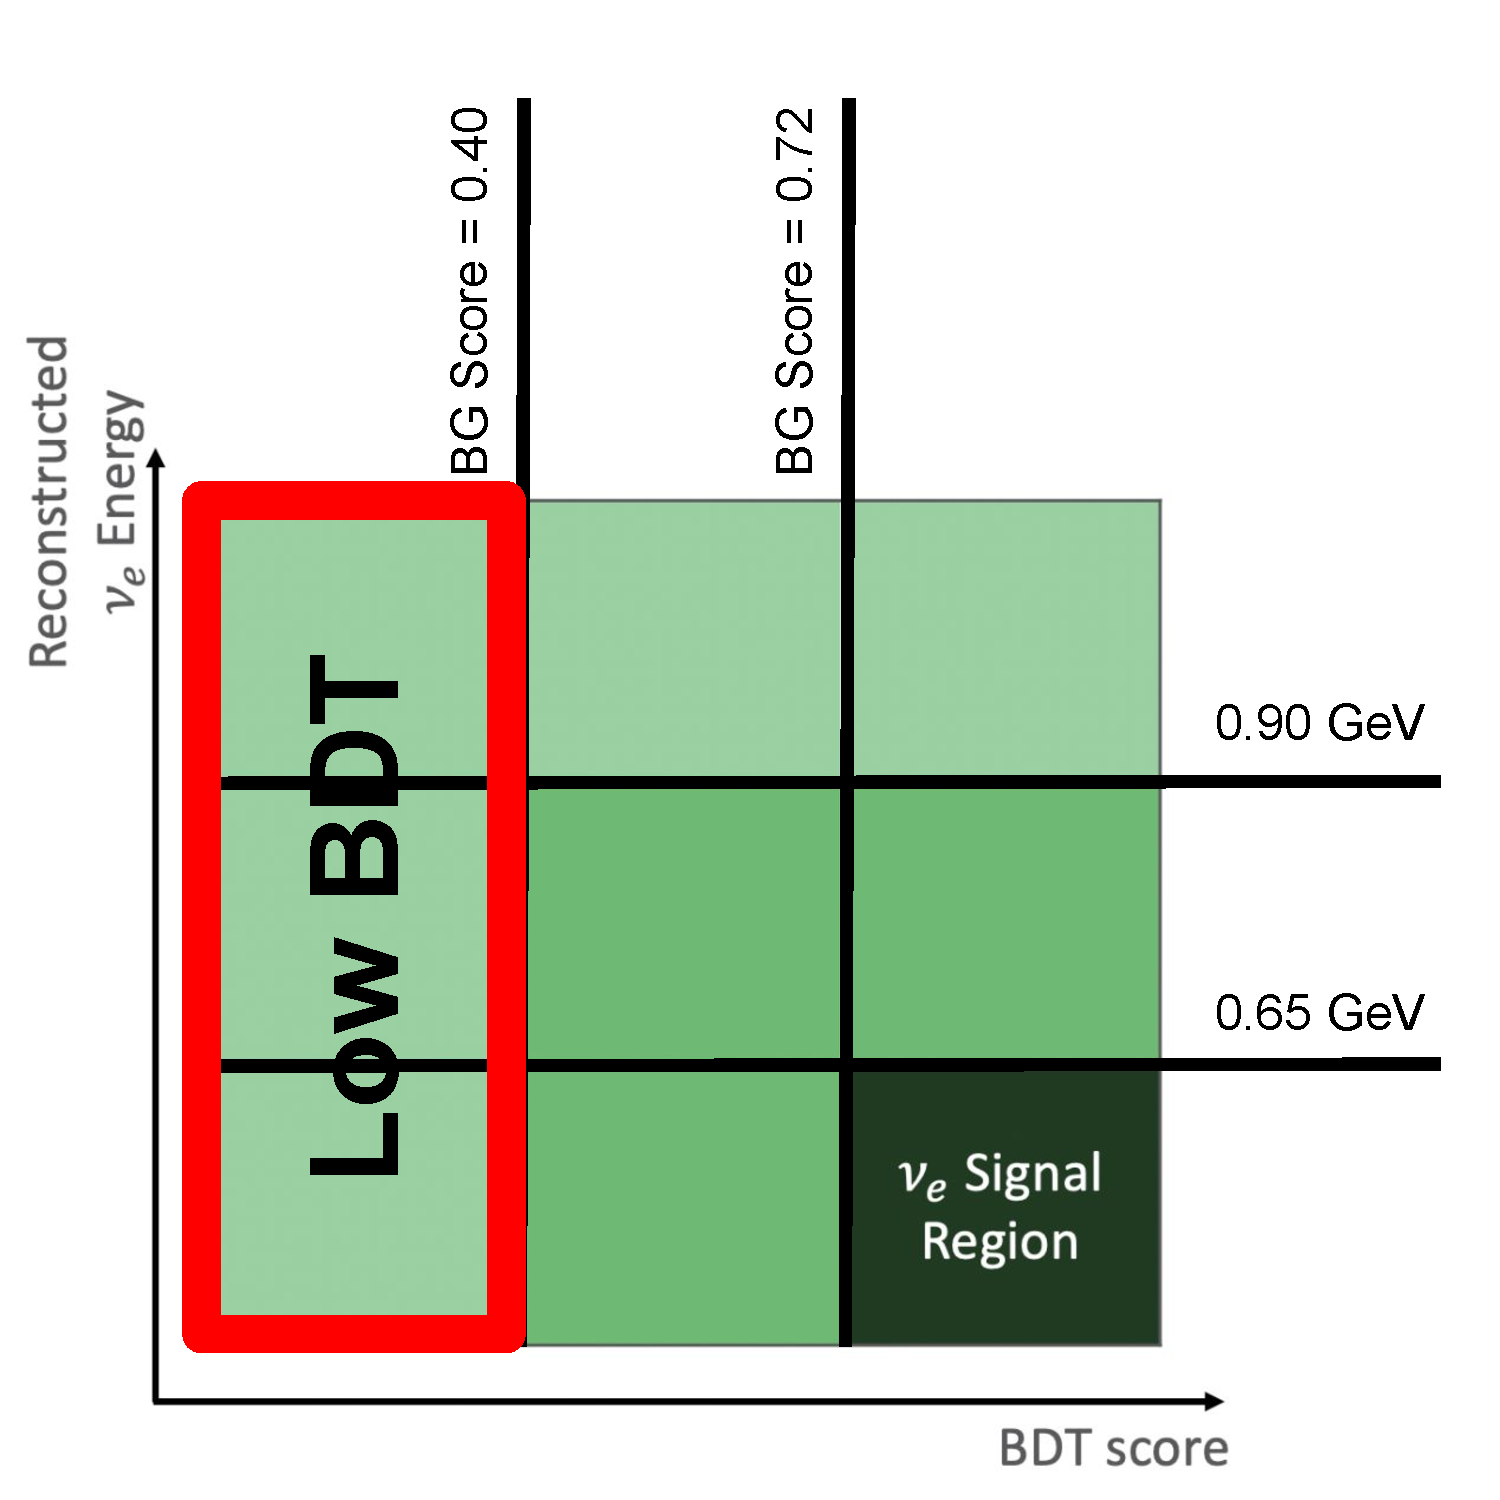
\includegraphics[width=\linewidth]{technote/Sidebands/Figures/FarSideband/ZpLowBDTSideband.pdf}
        \caption{For the 1e0p selection.}
    \end{subfigure}%
    \begin{subfigure}{0.5\linewidth}
        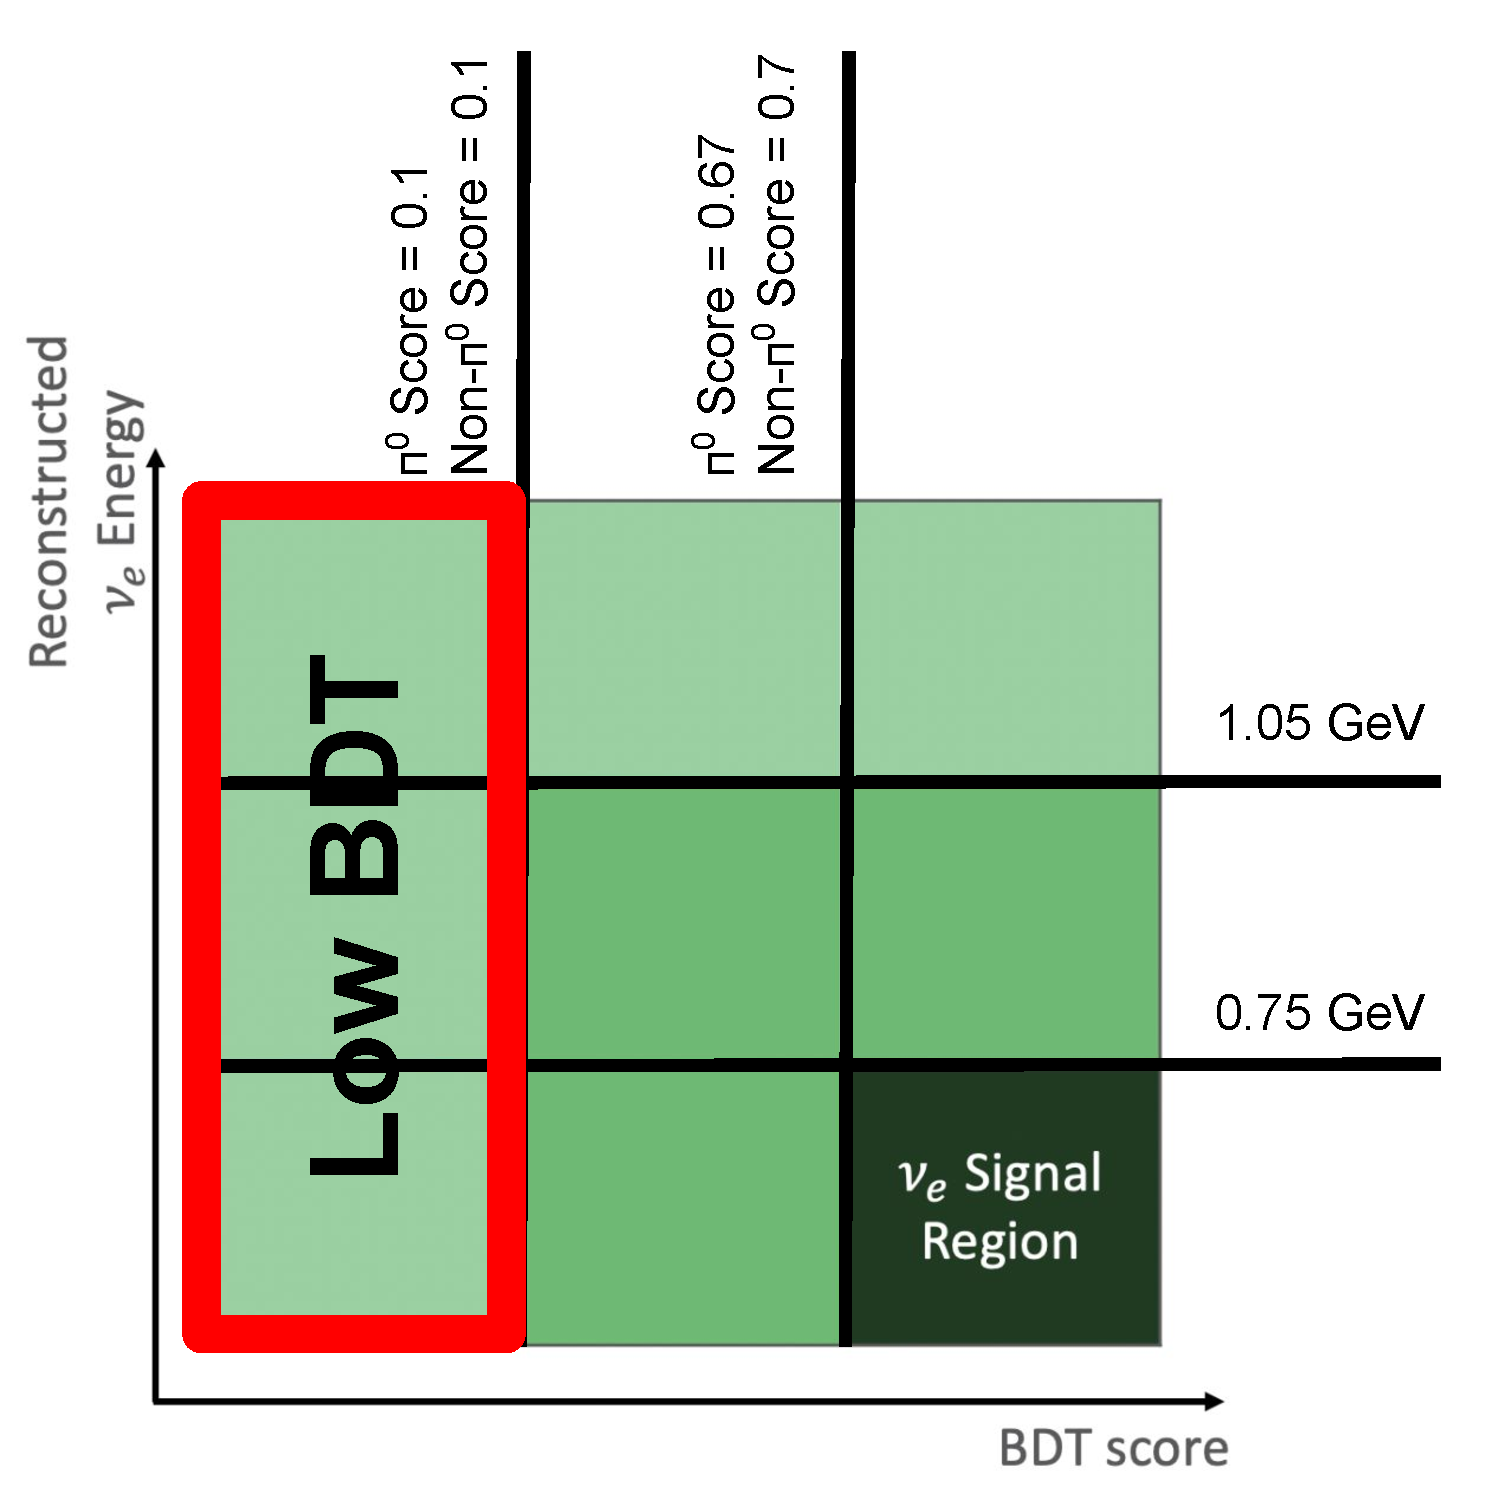
\includegraphics[width=\linewidth]{technote/Sidebands/Figures/FarSideband/NpLowBDTSideband.pdf}
        \caption{For the 1eNp selection.}
    \end{subfigure}
    \caption{The low BDT score sidebands.}
    \label{fig:LowBDTSideband}
\end{figure}

\begin{figure}[H]
    \centering
    \begin{subfigure}{0.5\linewidth}
        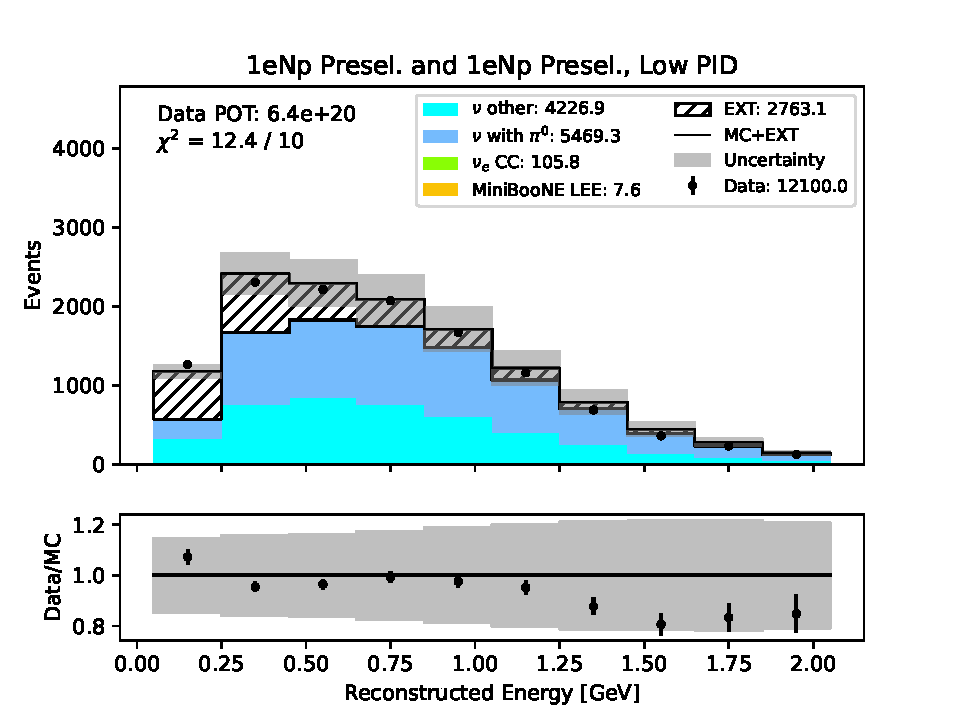
\includegraphics[width=\linewidth]{technote/Sidebands/Figures/FarSideband/far_sideband_reco_e_run123_NP_NP_LOW_PID.pdf}
        \caption{$\nu_e$ preselection, runs 1-3.}
    \end{subfigure}%
    \begin{subfigure}{0.5\linewidth}
        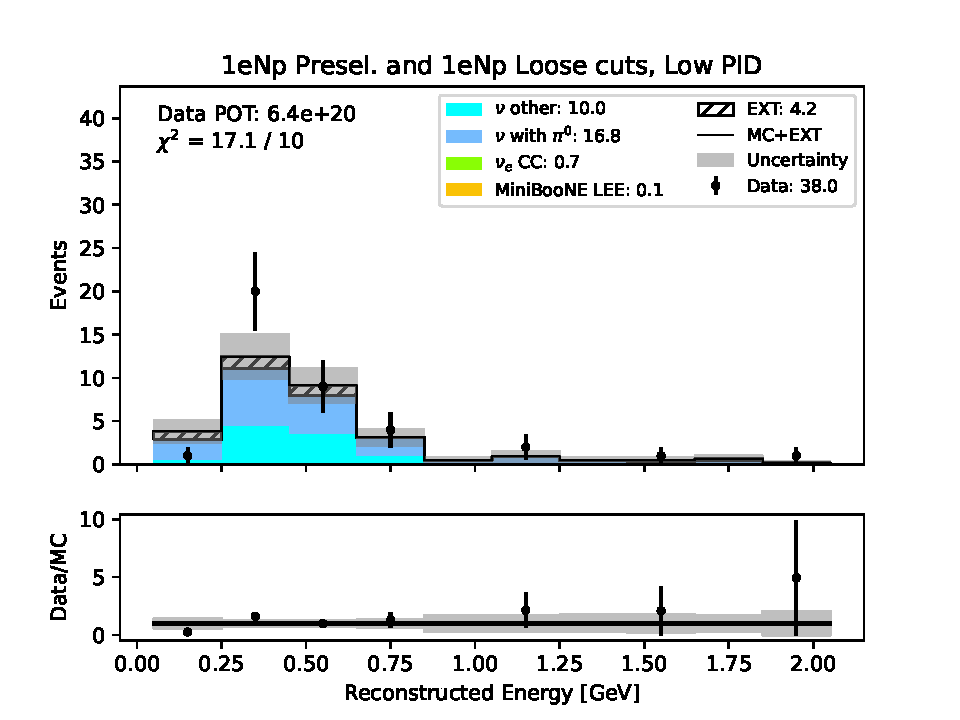
\includegraphics[width=\linewidth]{technote/Sidebands/Figures/FarSideband/far_sideband_reco_e_run123_NP_NPL_LOW_PID.pdf}
        \caption{1eNp loose selection, runs 1-3.}
    \end{subfigure}
    \begin{subfigure}{0.5\linewidth}
        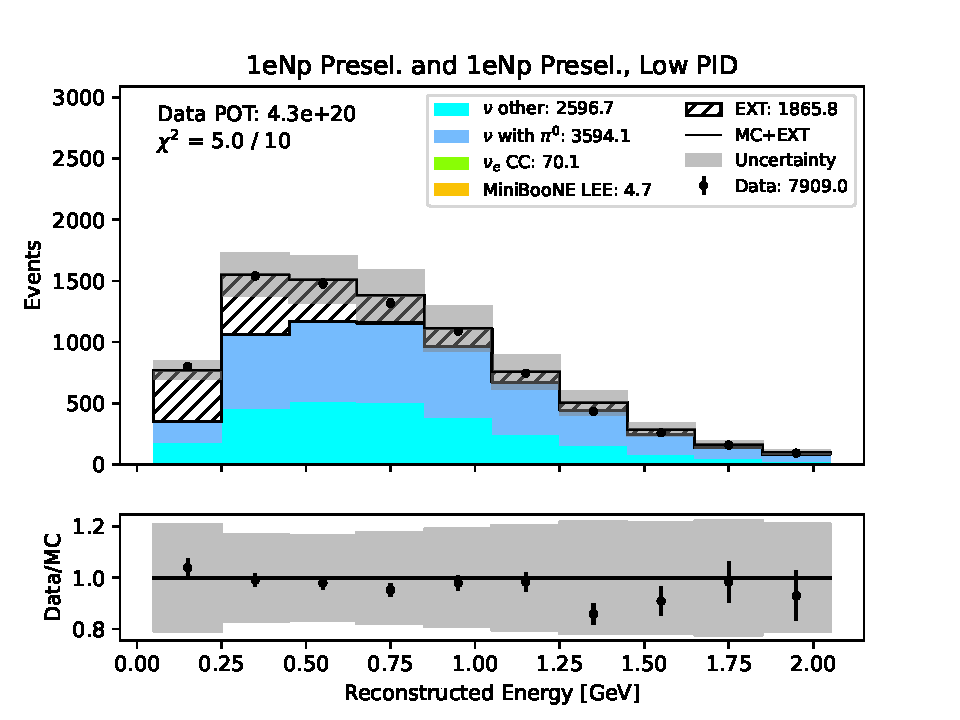
\includegraphics[width=\linewidth]{technote/Sidebands/Figures/FarSideband/far_sideband_reco_e_run4b4c4d5_NP_NP_LOW_PID.pdf}
        \caption{$\nu_e$ preselection, runs 4-5.}
    \end{subfigure}%
    \begin{subfigure}{0.5\linewidth}
        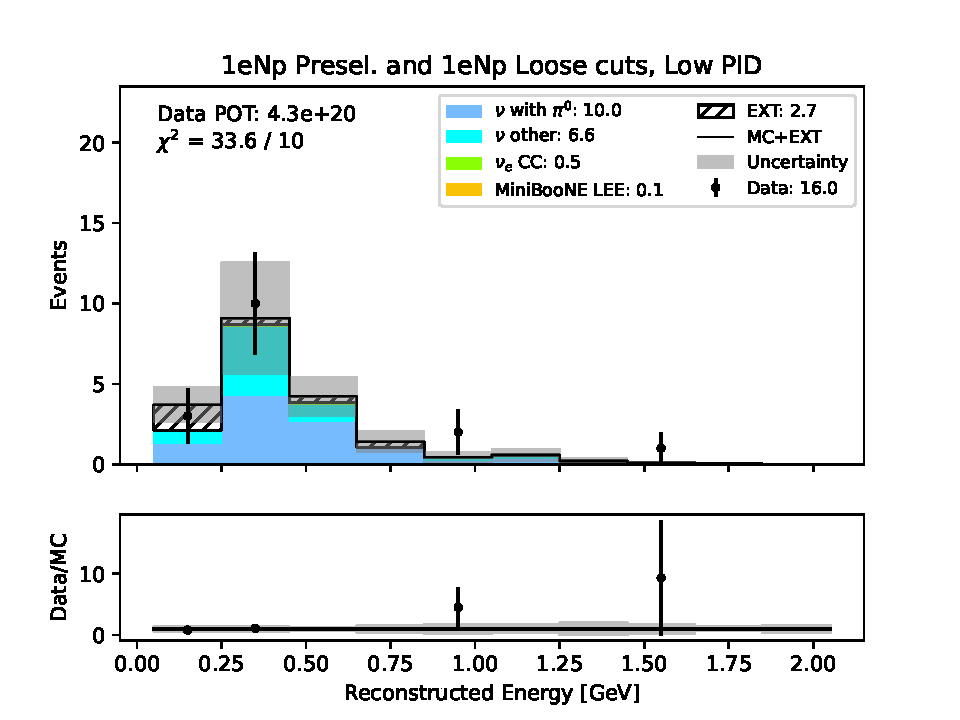
\includegraphics[width=\linewidth]{technote/Sidebands/Figures/FarSideband/far_sideband_reco_e_run4b4c4d5_NP_NPL_LOW_PID.pdf}
        \caption{1eNp loose selection, runs 4-5.}
    \end{subfigure}    
    \begin{subfigure}{0.5\linewidth}
        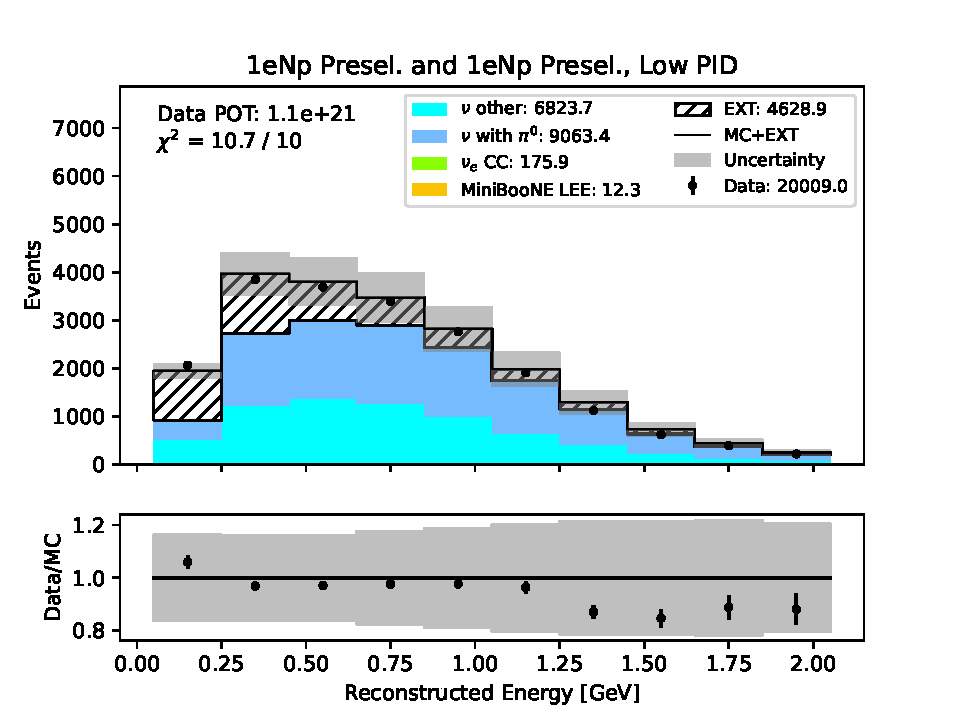
\includegraphics[width=\linewidth]{technote/Sidebands/Figures/FarSideband/far_sideband_reco_e_run1234b4c4d5_NP_NP_LOW_PID.pdf}
        \caption{$\nu_e$ preselection, runs 1-5.}
    \end{subfigure}%
    \begin{subfigure}{0.5\linewidth}
        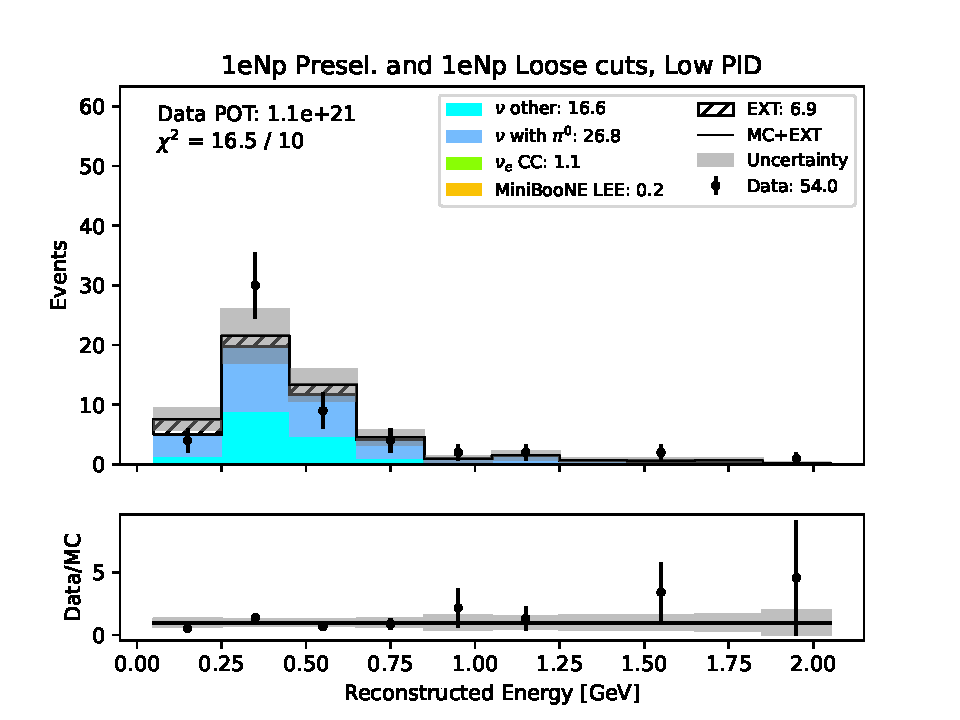
\includegraphics[width=\linewidth]{technote/Sidebands/Figures/FarSideband/far_sideband_reco_e_run1234b4c4d5_NP_NPL_LOW_PID.pdf}
        \caption{1eNp loose selection, runs 1-5.}
    \end{subfigure}
    \caption{Reconstructed neutrino energy using the low BDT score sideband and the 1eNp selections.}
\end{figure}

\begin{figure}
    \centering
    \begin{subfigure}{0.33\linewidth}
        \includegraphics[width=\linewidth]{technote/Sidebands/Figures/FarSideband/far_sideband_reco_e_run1_NP_NPL_LOW_PID.pdf}
        \caption{run 1.}
    \end{subfigure}%
    \begin{subfigure}{0.33\linewidth}
        \includegraphics[width=\linewidth]{technote/Sidebands/Figures/FarSideband/far_sideband_reco_e_run2_NP_NPL_LOW_PID.pdf}
        \caption{run 2.}
    \end{subfigure}%
    \begin{subfigure}{0.33\linewidth}
        \includegraphics[width=\linewidth]{technote/Sidebands/Figures/FarSideband/far_sideband_reco_e_run3_NP_NPL_LOW_PID.pdf}
        \caption{run 3.}
    \end{subfigure}
    \begin{subfigure}{0.33\linewidth}
        \includegraphics[width=\linewidth]{technote/Sidebands/Figures/FarSideband/far_sideband_reco_e_run4b_NP_NPL_LOW_PID.pdf}
        \caption{run 4b.}
    \end{subfigure}%
    \begin{subfigure}{0.33\linewidth}
        \includegraphics[width=\linewidth]{technote/Sidebands/Figures/FarSideband/far_sideband_reco_e_run4c_NP_NPL_LOW_PID.pdf}
        \caption{run 4c.}
    \end{subfigure}
    \begin{subfigure}{0.33\linewidth}
        \includegraphics[width=\linewidth]{technote/Sidebands/Figures/FarSideband/far_sideband_reco_e_run4d_NP_NPL_LOW_PID.pdf}
        \caption{run 4d.}
    \end{subfigure}%
    \begin{subfigure}{0.33\linewidth}
        \includegraphics[width=\linewidth]{technote/Sidebands/Figures/FarSideband/far_sideband_reco_e_run5_NP_NPL_LOW_PID.pdf}
        \caption{run 5.}
    \end{subfigure}
\end{figure}

\begin{figure}[H]
    \centering
    \begin{subfigure}{0.5\linewidth}
        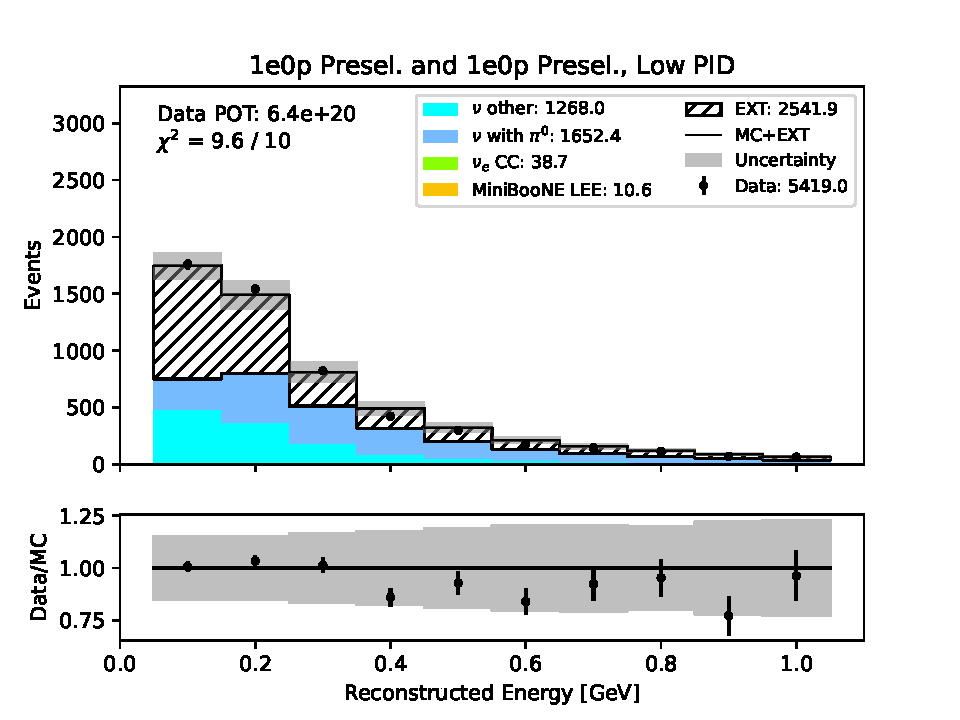
\includegraphics[width=\linewidth]{technote/Sidebands/Figures/FarSideband/far_sideband_reco_e_run123_ZP_ZP_LOW_PID.pdf}
        \caption{$\nu_e$ preselection, runs 1-3.}
    \end{subfigure}%
    \begin{subfigure}{0.5\linewidth}
        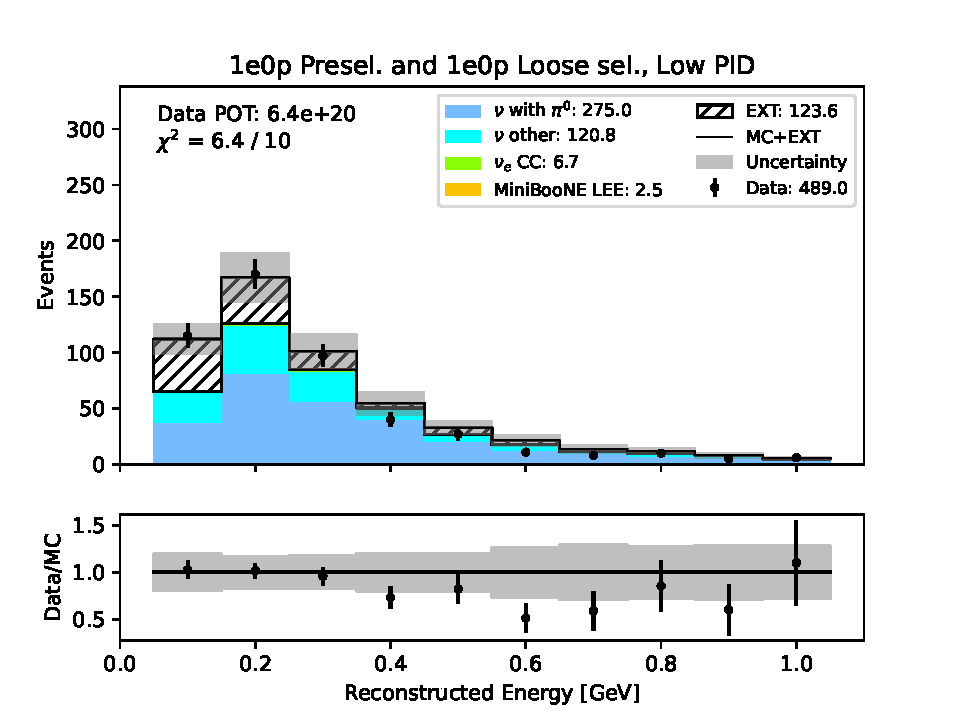
\includegraphics[width=\linewidth]{technote/Sidebands/Figures/FarSideband/far_sideband_reco_e_run123_ZP_ZPLOOSESEL_LOW_PID.pdf}
        \caption{1e0p loose selection, runs 1-3.}
    \end{subfigure}
    \begin{subfigure}{0.5\linewidth}
        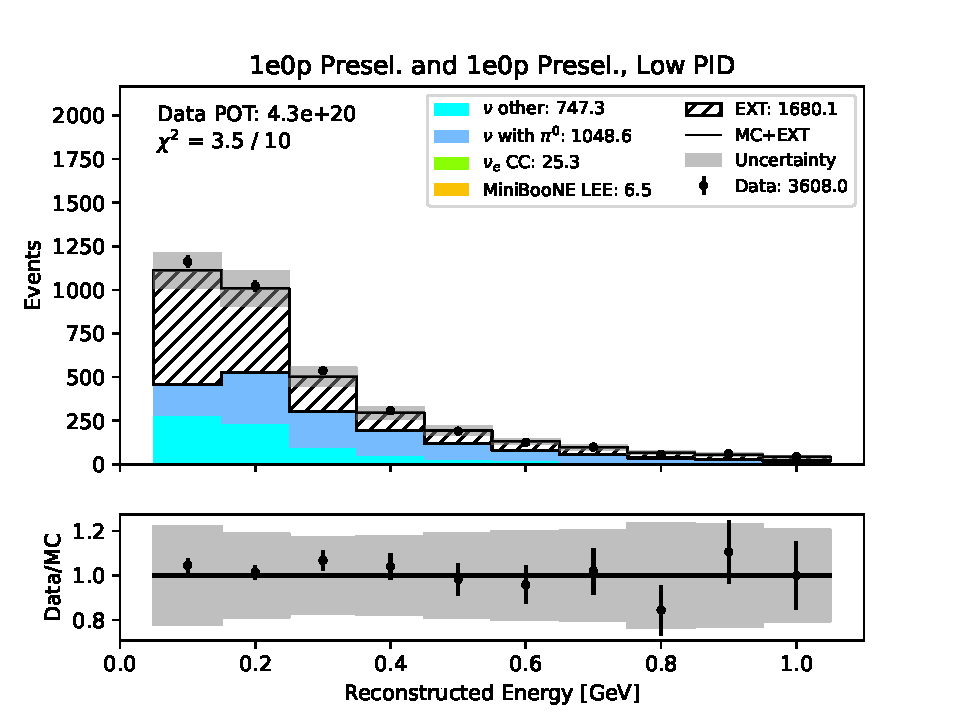
\includegraphics[width=\linewidth]{technote/Sidebands/Figures/FarSideband/far_sideband_reco_e_run4b4c4d5_ZP_ZP_LOW_PID.pdf}
        \caption{$\nu_e$ preselection, runs 4-5.}
    \end{subfigure}%
    \begin{subfigure}{0.5\linewidth}
        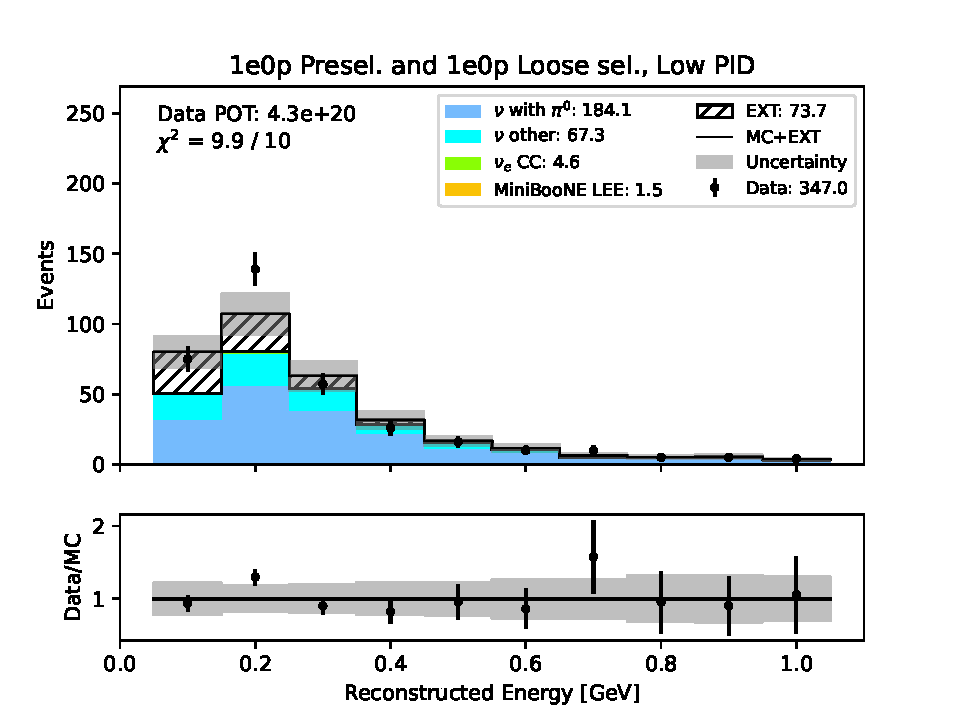
\includegraphics[width=\linewidth]{technote/Sidebands/Figures/FarSideband/far_sideband_reco_e_run4b4c4d5_ZP_ZPLOOSESEL_LOW_PID.pdf}
        \caption{1e0p loose selection, runs 4-5.}
    \end{subfigure}    
    \begin{subfigure}{0.5\linewidth}
        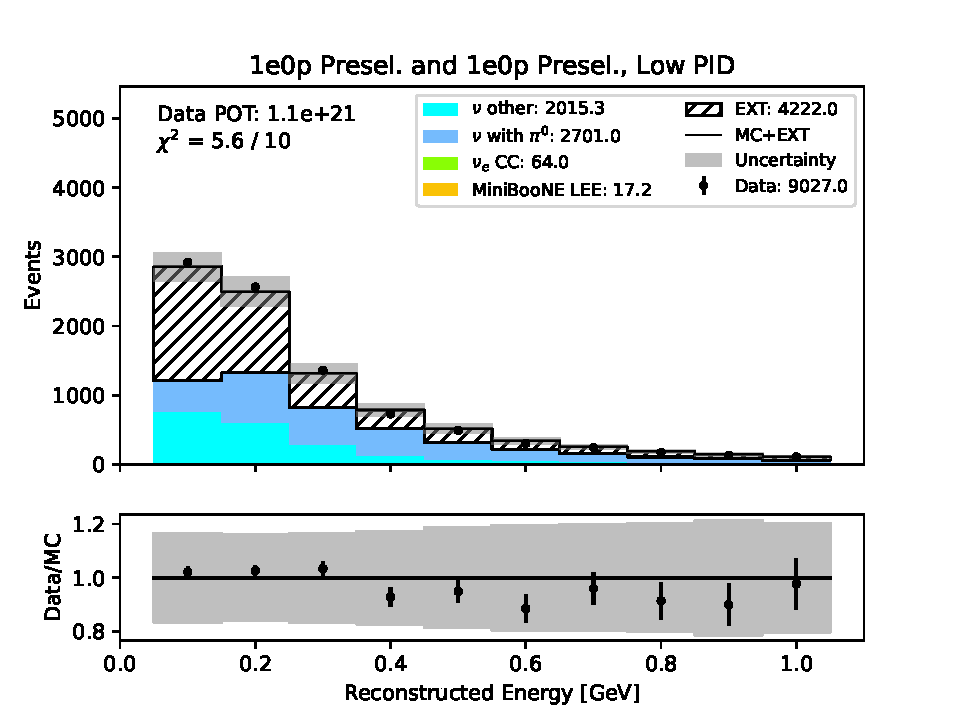
\includegraphics[width=\linewidth]{technote/Sidebands/Figures/FarSideband/far_sideband_reco_e_run1234b4c4d5_ZP_ZP_LOW_PID.pdf}
        \caption{$\nu_e$ preselection, runs 1-5.}
    \end{subfigure}%
    \begin{subfigure}{0.5\linewidth}
        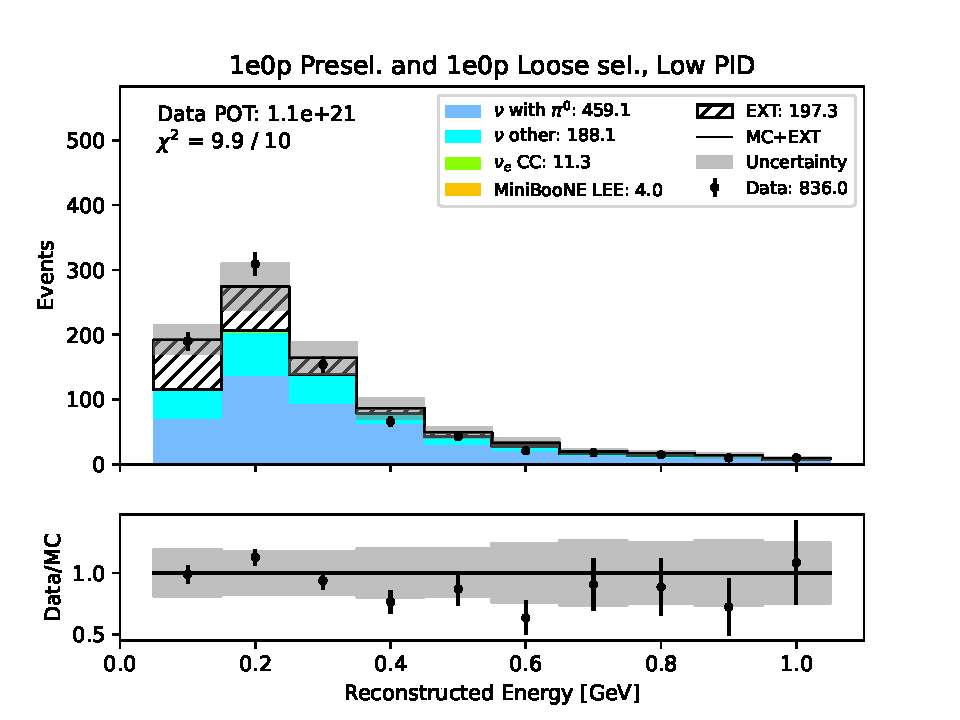
\includegraphics[width=\linewidth]{technote/Sidebands/Figures/FarSideband/far_sideband_reco_e_run1234b4c4d5_ZP_ZPLOOSESEL_LOW_PID.pdf}
        \caption{1e0p loose selection, runs 1-5.}
    \end{subfigure}
    \caption{Reconstructed neutrino energy using the low BDT score sideband and the 1e0p selections.}
\end{figure}
